\documentclass[12pt]{article}
\linespread{2}
\usepackage{times}
\usepackage{pgfplots}
\pgfplotsset{compat = newest}
\usetikzlibrary{positioning, arrows.meta}
\usepgfplotslibrary{fillbetween}
\usepackage{amsmath}
           \begin{document} 
                  \begin{center}
                        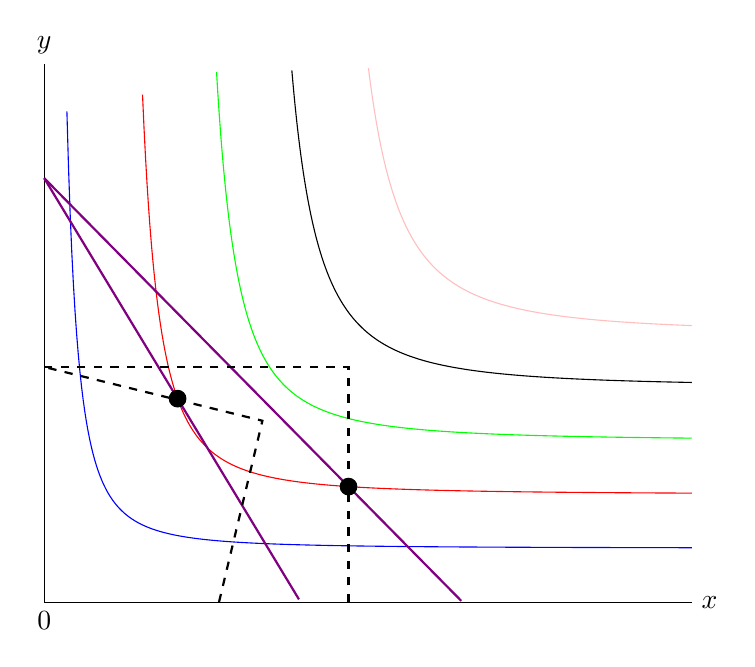
\begin{tikzpicture}
                              \begin{axis}[
                                           scale = 1.2,
                                           xmin = 0, xmax = 10,
                                           ymin = 0, ymax = 10,
                                           axis lines* = left,
                                           xtick = {0}, ytick = \empty,
                                           clip = false,
]
% Indifference curve
                       \addplot[domain = 0:10, restrict y to domain = 0:10, samples =
                                 400, color = blue]{1/(x^2)+1};
                       \addplot[domain = 1:10, restrict y to domain = 0:10, samples =
                                 400, color = red]{2/((x-1)^2)+2};
                       \addplot[domain = 2:10, restrict y to domain = 0:10, samples =
                                 400, color = green]{3/((x-2)^2)+3};
                       \addplot[domain = 3:10, restrict y to domain = 0:10, samples =
                                400, color = black]{4/((x-3)^2)+4};
                      \addplot[domain = 4:10, restrict y to domain = 0:10, samples =
                               400, color = pink]{5/((x-4)^2)+5};
% Labels 

                       \node [right] at (current axis.right of origin) {$x$};
                       \node [above] at (current axis.above origin) {$y$};
% Budget constraints
                       \addplot[domain = 0:10, restrict y to domain = 0:10, samples =
                                400, color = violet, thick]{7.88-1.22*x};
                       \addplot[domain = 0:10, restrict y to domain = 0:10, samples =
                                400, color = violet, thick]{7.88-1.99*x};  
                           
% dashed line segments                                
                        \addplot[color = black, dashed, thick] coordinates {(4.7, 0) (4.7,
                                 4.37) (0, 4.37)};
                        \addplot[color = black, dashed, thick] coordinates {(2.7, 0) (3.37,
                                 3.37) (0, 4.37)};
% coordinate points
                                 
                        \addplot[color = black, mark = *, only marks, mark size = 3pt]
                                 coordinates {(2.06, 3.781) (4.7, 2.146)};
                \end{axis}
           \end{tikzpicture}
      \end{center}
               \textbf{Figure 07}
  \end{document} 